\section{Initial Problem}\label{sec:initproblem}
Wearable technology is a trending form of technology as of 2015 \cite{WEARABLESTREND}. 
As the name implies, wearables are devices that, 
unlike most electronics, are worn by the user. 
As shown by \Cref{fig:wearables-placement}, 
the most common type of wearables today are wrist-worn, 
\eg smartwatches or smart-wristbands (such as fitness trackers).
Smartwatches are watches that run an advanced operating system, 
and can perform more actions than regular watches, 
such as communicating with a smartphone or other smart devices.
Smart-wristbands are typically fitness trackers which track activity, among other things, 
and send this data to a connected smartphone via an application. 
Smartphones are usually not considered a wearable since they are \emph{carried} and not \emph{worn}. 

\begin{figure}[!htb]
  \centering
  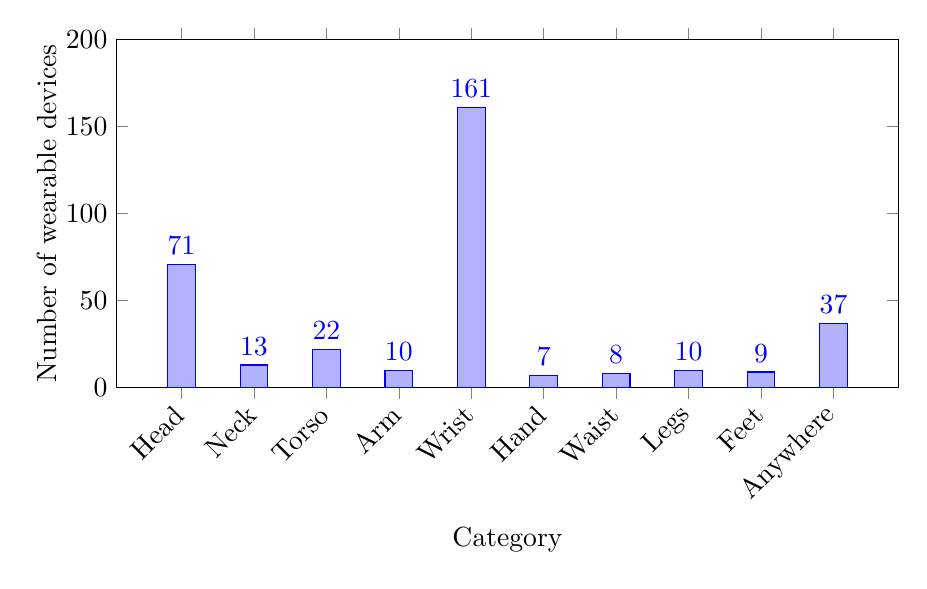
\begin{tikzpicture}
\begin{axis}[
    height=6cm,
    width=0.95\textwidth,
    xlabel={Category},
    xticklabel style={rotate=45, anchor=east, yshift=-0.5ex},
    ylabel={Number of wearable devices},
    yticklabel style={align=right,inner sep=0pt,xshift=-0.3em},
    nodes near coords align={vertical},
    nodes near coords,
    xtick=data,
    symbolic x coords={Head,Neck,Torso,Arm,Wrist,Hand,Waist,Legs,Feet,Anywhere},
    ybar,
    ymax=200,
    ymin=0,
    ]
    \addplot coordinates {(Head,71) (Neck,13) (Torso,22) (Arm,10) (Wrist,161) (Hand,7) (Waist,8) (Legs,10) (Feet,9) (Anywhere,37)};
\end{axis}
  

\end{tikzpicture}
  \caption{Placements of wearables. Data from \protect\cite{LISTOFWEARABLES}.}
  \label{fig:wearables-placement}
\end{figure}

The increasing trend in wearables is likely due to increased computational power in small devices, 
and decreased sizes of sensors, 
which allows more power and functionality to wearables devices. 
This increasing trend, as well as better wearables devices, 
opens up new possibilities since we can now carry more computational power with us on the go, 
which we can utilize to perform actions that we could not before, 
or perform actions faster or better. 
An example of this is that we can now track our level of activity, 
together with our location to analyze ourselves, 
or even automate actions based on our location, mood or even health. 

Another trend that utilizes IoT is smart homes.
Smart homes are homes that are to some degree automated by utilizing IoT devices. 
The devices used for smart homes differ from wearables as they are usually stationary. 
The concept of smart homes has been around since the 1960's, 
where ``wired homes'' were built by hobbyists\cite{harper2003}. 
The first official use of ``Smart house'' was in 1984, 
by the American Association of Housebuilders \cite{harper2003}.

An extreme example of a high-end smart home is Bill Gate's mansion in Medina, Washington \cite{billgatehouse}.
This \$100 million house, finished in 2005, 
has sensors to adjust each room's temperature and lighting, 
and has speakers behind the wallpaper that follow you from room to room. 
The artwork in the house is mostly digital and can be changed by pressing a button. 
One can only imagine what other technology is being used in that house. 

With these increasing technology trends in wearables and smart homes, 
it could be very interesting to see how and if we can integrate these. 
It could be interesting to see if we can use wearables as a form of control of smart homes, 
or maybe even use wearables to automate the smart homes.
In the following sections we will look into the current state of wearables and smart homes, 
and investigate if we can integrate them. 
